\documentclass[12pt, a4paper]{article}
\usepackage[a4paper, margin=2cm]{geometry}
\usepackage{graphicx} 
\usepackage{multirow}
\graphicspath{{../}}

\title{Trustworthy Machine Learning - EX1}
\author{Ishay Yemini}
\date{\today}

\begin{document}
\maketitle

\section{White-box vs. query-based black-box attack}

\begin{enumerate}
  \item The benign accuracy of the model is 87.5\%.
  \item Untargeted success rate: 98.5\%. \\ 
  Targeted success rate: 94.5\%.
  \item The success rates for the Black-Box untargeted and targeted attacks are presented in table \ref{tab:bbox}. We can clearly see that these attacks are not as successful as the White-Box attack from the last subsection. This aligns with our expectation, as the White-Box attack is able to use the real gradient, while the Black-Box attack can only use an estimate of it. \\
  Additionally, momentum improves the success rate and lowers the number of queries needed, for both untargeted and targeted attacks. This maybe happens because the momentum causes the algorithm to use the gradients from the previous iterations, thereby making the estimation less noisy than without momentum. This allows for better convergence, which results in higher success rates and less queries, as our results show. \\
  The box plots from our experiment are present in figures \ref{fig:bbox-untargeted} and \ref{fig:bbox-targeted}.
\end{enumerate}


\begin{figure}[hbt]
  \centering
  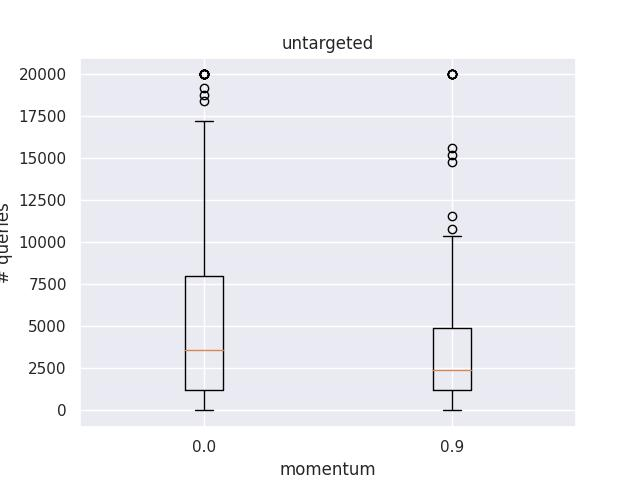
\includegraphics[width=0.6\textwidth]{bbox-n_queries_untargeted}  
  \caption{Black-box untargeted number of queries}
  \label{fig:bbox-untargeted}
\end{figure}

\begin{figure}[hbt]
  \centering
  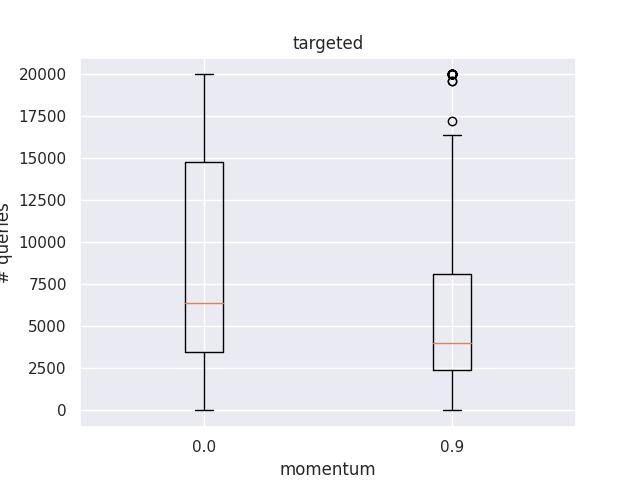
\includegraphics[width=0.6\textwidth]{bbox-n_queries_targeted}  
  \caption{Black-box targeted number of queries}
  \label{fig:bbox-targeted}
\end{figure}

\begin{table}[hbt]
  \begin{center}
    \begin{tabular}{|c|c|c|c|}
      \hline
    Type & Momentum & Success Rate & Queries \\
      \hline
    Untargeted & 0 & 93\% & 3,600\\
      \hline
    Targeted & 0 & 81\% & 6,400\\
      \hline
    Untergeted & 0.9 & 96.5\% & 2,400\\
      \hline
    Targeted & 0.9 & 88\% & 4,000\\
      \hline
    \end{tabular}
    \caption{Black-box attacks success rates and number of queries}
  \end{center}
  \label{tab:bbox}
\end{table}


\section{Transferability-based black-box attack.}

We can see that untargeted attacks transfer much better than targeted attacks, as presented in tables 2 and 3. \\
When using an ensemble attack, trained on models 1 and 2, we get much better results: for the untargeted attack we get a success rate of 74\%, much better than the 55.5\%-54\% we got with only one of 1 or 2. Similarly, we for the targeted attack we get a success rate of 50\% - almost two times better than the 25.5\% we got with only a single model! \\
This can be explained by the fact that now, the attack is less susceptible to specificities in different models, and by training on two models, this smoothes out the PGD process, thus finding features that generalize better. 

\begin{table}[hbt]
  \begin{center}
    \begin{tabular}{|c|c||c|c|c|}
      \cline{3-5}
    \multicolumn{2}{c||}{} & \multicolumn{3}{|c|}{Attacked} \\
      \cline{3-5}
    \multicolumn{2}{c||}{} & 0 & 1 & 2 \\
      \hline \hline
    & 0 & 98.5\% & 55.5\% & 54\%\\
      \cline{2-5}
    Trained & 1 & 68.5\% & 96.5\% & 58.5\%\\
      \cline{2-5}
    & 2 & 60\% & 54.5\% & 95.5\%\\
      \hline
    \end{tabular}
    \caption{Untargeted attacks' transferability.}
  \end{center}
  \label{tab:ut-trans}
\end{table}

\begin{table}[hbt]
  \begin{center}
    \begin{tabular}{|c|c||c|c|c|}
      \cline{3-5}
    \multicolumn{2}{c||}{} & \multicolumn{3}{|c|}{Attacked} \\
      \cline{3-5}
    \multicolumn{2}{c||}{} & 0 & 1 & 2 \\
      \hline \hline
    & 0 & 92.5\% & 25.5\% & 25.5\%\\
      \cline{2-5}
    Trained & 1 & 37\% & 89.5\% & 27\%\\
      \cline{2-5}
    & 2 & 32.5\% & 23.5\% & 84\%\\
      \hline
    \end{tabular}
    \caption{Targeted attacks' transferability.}
  \end{center}
  \label{tab:t-trans}
\end{table}


\section{Bit-flip attacks}

\begin{enumerate}
  \item The maximum RAD is 74.55\%. 
  \item The fraction of bits that lead to $>15\%$ RAD when flipped is 0.0213 bits. 
  \item We can see in figure \ref{fig:bf} that bit 1 has the highest median RAD. This makes sense: bit 0 is the sign bit, so bit 1 is the MSB, so flipping it is expected to have the most effect on the parsed float. 
\end{enumerate}

\begin{figure}[hbt]
  \centering
  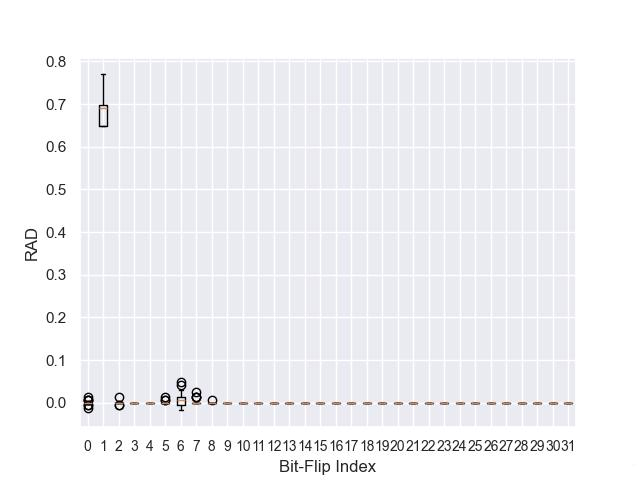
\includegraphics[width=0.6\textwidth]{bf_idx-vs-RAD}  
  \caption{Bit-Flip index vs. RAD}
  \label{fig:bf}
\end{figure}


\end{document}

